\section{Numerical results}\label{sec:results}
\subsection{Finite-block predictions and approximation errors}
Figure~\ref{fig:revision-benchmark} and
Table~\ref{tab:revision-validation} compare the population calculation
with independent block samples. Across $64$ configurations, $61$ nominal
$95\%$ intervals contain the predicted inflation, and the largest point
discrepancy is $4.66\%$. The three misses are lognormal $(n,L)=(128,2)$,
exponential $(8,2)$, and Beta$(2,5)$ $(32,2)$.

% Generated from experiments/tables.tex
\begin{table}[t]
\centering\footnotesize
\caption{New finite-$n$ validation at $L=2$, $n=4096$. Monte Carlo brackets are 95\% block-bootstrap intervals; Pareto uses conditional stratification. $\mathcal I_{\mathrm{drop}}$ drops only $c_k$ while retaining exact conditional one-element moments; $\mathcal I_{\mathrm{red}}$ additionally replaces those moments by unconditional responses.}\label{tab:revision-validation}
\begin{tabular}{@{}lrrrr@{}}\toprule
Distribution & MC [95\% CI] & Exact & $\mathcal I_{\mathrm{drop}}$ & $\mathcal I_{\mathrm{red}}$\\\midrule
Gaussian & 1.013 [0.965, 1.056] & 1.000 & 1.000 & 1.000\\
Half-normal & 14.86 [14.50, 15.19] & 14.927 & 14.927 & 14.905\\
ReLU & 6.202 [5.913, 6.483] & 6.205 & 6.205 & 6.186\\
Lognormal & 173.8 [168.0, 178.8] & 177.1 & 177.1 & 177.3\\
Pareto(4) & 2893.7 [2893.0, 2894.7] & 2894.1 & 2894.1 & 2895.0\\
Exponential & 41.78 [39.99, 43.73] & 41.794 & 41.794 & 41.794\\
\bottomrule\end{tabular}
\end{table}

% Generated from experiments/figures.tex
\begin{figure}[t]
\centering
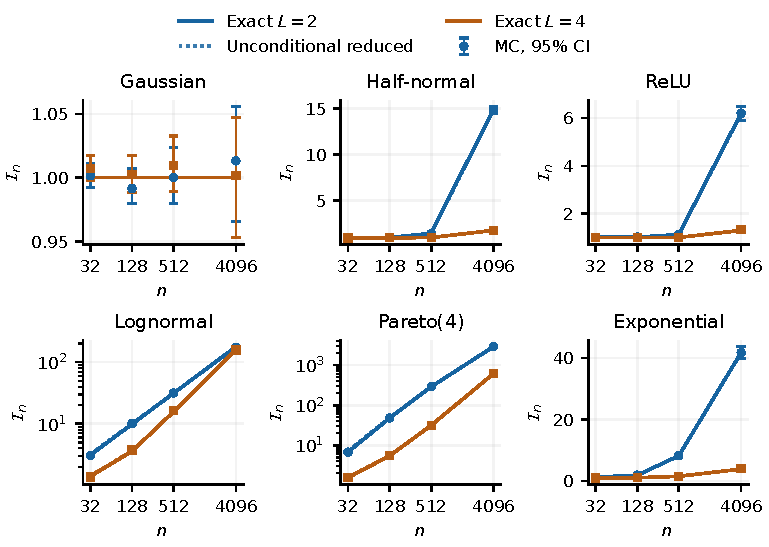
\includegraphics[width=\linewidth]{revision/experiments/figure_benchmark.pdf}
\caption{Finite-block validation on six input laws. Solid curves are exact moment predictions; dotted curves use unconditional responses and drop conditional covariance. Markers show Monte Carlo estimates with 95\% intervals, using conditional stratification for Pareto.}\label{fig:revision-benchmark}
\end{figure}


For asymmetric laws at $n=4096$, $L=2$, the predicted inflation is
$6.205$ for ReLU, $14.927$ for half-normal, $177.1$ for lognormal,
$41.794$ for exponential, and $2894.1$ for Pareto$(4)$.
Changing the precision changes which binades place most inputs in the
zero cell, producing distinct block-length trends.
The conditional-mean upper prediction has maximum additive excess
$0.00648$ in the continuous-law grid. The unconditioned-response
approximation instead has maximum relative discrepancy $5.81\%$,
at Pareto$(4)$, $n=32$, $L=2$: exact inflation is $6.806$, the
conditional-mean upper value is $6.812$, and the unconditioned-response
value is $7.201$. The dominant approximation error here is in the
conditional marginal moments.

Pareto inputs expose the importance of rare scale states. Ordinary
sampling differs from the population prediction by as much as $14.8\%$;
sampling every retained exponent stratum brings all eight predictions
within their intervals. The omitted marginal second-moment bound is
$3.0\times10^{-8}$ at $L=2$ and $1.9\times10^{-9}$ at $L=4$.
Both sampling records are retained.

\paragraph{Rounding controls.}
All eight stochastic-rounding inflation intervals contain one.
At $n=128$, $L=2$, the Gaussian marginal-variance ratio
$12\widehat v/\widehat{\mathbb E[s^2]}$ is approximately $1.000$
for round-to-nearest and $2.000$ for stochastic rounding.
For ReLU, the atom at zero contributes zero error; the ratios are
approximately $1/2$ and $1$, respectively.
These controls check the symmetric residual, conditional unbiasedness,
and treatment of atoms.

\subsection{Weighted reductions and block partition}
For $n=128$, $L=2$, we use positive weights, alternating $1,-1$,
and alternating $1,-0.9$. Define
\begin{equation}\label{eq:weight-imbalance}
 \chi=\frac{(\mathbf1^Tw)^2}{n\|w\|_2^2}\in[0,1].
\end{equation}
Equation~\eqref{eq:revision-weighted} gives
$\mathbb E[E_w^2]/\|w\|_2^2=(v-\kappa)+n(\kappa+\mu^2)\chi$.
The three vectors have $\chi=1$, $0$, and approximately $0.00276$.
Figure~\ref{fig:revision-weighted} and Table~\ref{tab:revision-weighted}
compare shared-scale rounding, split blocks, and independently selected
scales. The predictions have maximum MSE discrepancy $1.48\%$; eleven
of twelve nominal intervals contain them.

% Generated from experiments/tables.tex
\begin{table}[t]
\centering\footnotesize
\caption{Weighted dot-product quantization MSE divided by $\sum_iw_i^2$, lognormal inputs, $n=128$, $L=2$, 50,000 blocks. Brackets are 95\% intervals. The weights are fixed before sampling. Balanced: alternating $1,-1$; near cancellation: alternating $1,-0.9$; positive: all ones.}\label{tab:revision-weighted}
\begin{tabular}{@{}lrrr@{}}\toprule
Method & Balanced & Near cancellation & Positive\\\midrule
Shared RNE & 0.509 [0.500, 0.517] & 0.545 [0.535, 0.555] & 12.58 [12.40, 12.80]\\
Split blocks of 16 & 0.165 [0.162, 0.167] & 0.166 [0.164, 0.168] & 0.816 [0.805, 0.827]\\
Independent scales & 0.020 [0.020, 0.021] & 0.020 [0.020, 0.021] & 0.023 [0.023, 0.024]\\
Shared SR & 1.375 [1.345, 1.407] & 1.374 [1.348, 1.404] & 1.380 [1.350, 1.413]\\
\bottomrule\end{tabular}
\end{table}

% Generated from experiments/figures.tex
\begin{figure}[t]
\centering
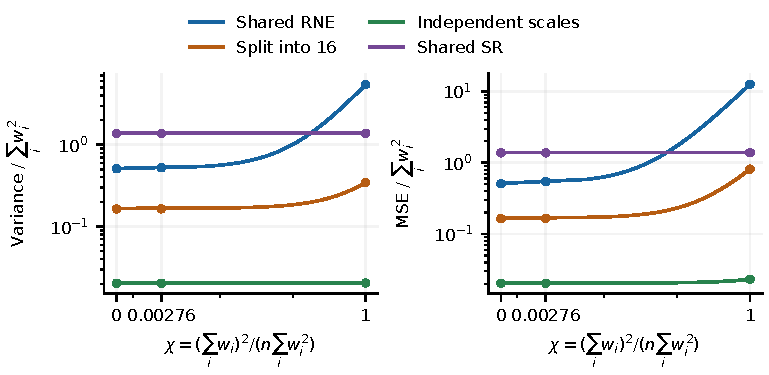
\includegraphics[width=\linewidth]{revision/experiments/figure_weighted.pdf}
\caption{Weighted dot products for lognormal inputs ($n=128$, $L=2$). Fixed weights vary the normalized imbalance $\chi=(\sum_iw_i)^2/(n\sum_iw_i^2)\in[0,1]$. Curves evaluate the affine laws from exact moments on a dense grid; markers show Monte Carlo with 95\% intervals.}\label{fig:revision-weighted}
\end{figure}


Shared round-to-nearest gives normalized MSE $12.58$ for positive
weights and $0.509$ for balanced weights. For positive weights,
centered variance is about $695.1$ and MSE is $1610.0$, showing the
additional squared-bias contribution. Stochastic rounding gives
normalized MSE near $1.38$ for both patterns: eliminating bias and
covariance improves the positive reduction, while its larger marginal
variance worsens the balanced reduction.
Splitting into length-$16$ blocks gives positive-weight MSE $0.816$;
an independent scale per coordinate gives $0.023$. The following
elliptic experiments account for the storage cost of those scale choices.

\paragraph{Asymptotic verification.}
Table~\ref{tab:revision-exponential} evaluates the subsequence in
Theorem~\ref{thm:revision-exponential} at $L=2$, $j=3,\ldots,8$.
Cell integration at $100$ and $160$ digits and the closed exponential
formula agree in all displayed digits. Inflation grows from about $41$
to $4.558\times10^{99}$, while the final $\mathcal I_n/n$ is
$3.016\times10^{-12}$ and the ratio to the theorem normalization is
$0.99999955$.
Here $\mathcal I_n$ is a centered variance ratio; it is not the absolute
mean-square error, whose additional coherent-bias term is given in
\eqref{eq:revision-weighted}. The high-precision calculation resolves
population-moment cancellation and does not claim that a binary64 reduction
would form the displayed sum without overflow or loss of significance.
% Generated from experiments/tables.tex
\begin{table}[t]
\centering\footnotesize
\caption{Exact high-precision exponential counterexample at $L=2$, $n=\lfloor e^{2^j}\rfloor$. The theorem normalization is $C(\log n)^2 n^{7/8}$ with $C=e^{-1}(1-e^{-1})/64$. Convergence of the ratio to one is predicted by the asymptotic theorem. All displayed values agree between 100 and 160 decimal digits.}\label{tab:revision-exponential}
\begin{tabular}{@{}rrrr@{}}\toprule
$2^j$ & $\mathcal I_n$ & $\mathcal I_n/n$ & Exact / normalization\\\midrule
8 & $4.111\times10^{1}$ & $1.380\times10^{-2}$ & 0.161276\\
16 & $3.296\times10^{5}$ & $3.709\times10^{-2}$ & 0.294655\\
32 & $3.298\times10^{12}$ & $4.177\times10^{-2}$ & 0.612870\\
64 & $2.901\times10^{25}$ & $4.652\times10^{-3}$ & 0.931787\\
128 & $2.601\times10^{50}$ & $6.690\times10^{-6}$ & 0.998663\\
256 & $4.558\times10^{99}$ & $3.016\times10^{-12}$ & 1.000000\\
\bottomrule\end{tabular}
\end{table}


\subsection{Spatially heterogeneous sources in an elliptic solve}
\label{sec:revision-elliptic2d}
Consider $-\Delta u=f$ on $(0,1)^2$ with homogeneous Dirichlet conditions.
On an $m\times m$ interior grid, let $h=(m+1)^{-1}$,
$A=h^{-2}(I\otimes T+T\otimes I)$ with
$T=\operatorname{tridiag}(-1,2,-1)$, and $G=A^{-1}$.
We compress the cell sources $b_i=s_i\exp(Z_i)$, where the $Z_i$ are
independent $N(0,1)$ variables. The prescribed spatial scales are
\begin{align*}
 s_{\rm sm}(x,y)&=1+3\sin^2(\pi x)\sin^2(\pi y),\\
 s_{\rm hot}(x,y)&=1+7\exp\!\left(-\frac{(x-0.3)^2+(y-0.65)^2}{0.02}\right).
\end{align*}
These profiles test the nonidentical-input formula with smooth variation
and a localized source hotspot.

Write $e=Q(b)-b$, $\delta u=Ge$, $\mu=\mathbb E e$, and
$\Sigma_B=\operatorname{Cov}(e_B)$ for a partition into disjoint blocks.
For any symmetric positive definite $A$, define $\|z\|_{A,h}^2=h^2z^TAz$.
Independence across blocks gives
\begin{equation}\label{eq:revision-elliptic2d-energy}
 J:=\mathbb E\|\delta u\|_{A,h}^2
 =h^2\left[\sum_B\operatorname{tr}(G_{BB}\Sigma_B)
                 +\mu^TG\mu\right].
\end{equation}
The bias term couples different spatial blocks. Relative RMS is
$\sqrt{J/\{h^2\mathbb E[b^TGb]\}}$, with the denominator evaluated
from the source laws. The baseline denoted Ind. retains every exact
marginal mean and variance while dropping off-diagonal error covariances;
Unif. uses independent zero-mean uniform-cell errors.

All codecs pack exactly $7m^2$ payload bits: an 8-bit signed exponent per
block, $L_B+3$ signed bits per coefficient, and any remaining padding.
Block lengths are $8,32,128$, with contiguous and interleaved layouts.
The largest common precision is supplemented by prescribed extra-bit
blocks. Their locations are fixed codec maps, so no data-dependent flags
are needed. At $m=32$, we compare evenly spaced locations (Uniform),
descending $\sum_{i\in B}s_i^2$ (Source), and a greedy full-energy rule
(Energy). For a candidate precision increment, embed its mean change
$d$ in the full vector and let $\Delta\Sigma_B$ be its block covariance
change. The greedy rule chooses the smallest
\begin{equation}\label{eq:revision-elliptic2d-increment}
 \Delta J=h^2\left[\operatorname{tr}(G_{BB}\Delta\Sigma_B)
                     +2d^TG\mu+d^TGd\right].
\end{equation}
Ties are resolved by block index. The implemented codec rejects
out-of-range exponents; none occurred, and the per-vector probability
bound is below $10^{-1632}$.

We retain all $40$ prescribed configurations, including coincident
precision maps, and use $20\,000$ paired source vectors per profile for
$m=16$ and $60\,000$ for $m=32$, with $300$ whole-vector bootstrap
replicates. The latter pools the initial $10\,000$ vectors and a declared
independent $50\,000$-vector replication for both profiles. All streams,
configuration records, and interval misses remain in the package.
The primary nominal intervals contain 34 of $40$ population RMS predictions;
the largest RMS discrepancy is 0.83\%.

\begin{table}[tb]
\centering
\caption{Two-dimensional heterogeneous source compression, $32^2$ unknowns,
contiguous blocks, and exactly $7168$ payload bits. Source and Energy allocate
the extra coefficient bits by source scale and the full energy prediction,
respectively. Relative energy RMS values are percentages. Ind. retains exact
marginal moments and bias; Unif. uses independent uniform-cell noise.}
\label{tab:revision-elliptic2d}
\begingroup\footnotesize\setlength{\tabcolsep}{3pt}
\begin{tabular}{lrlrrrr}
\toprule
Profile & $|B|$ & Placement & Exact & Ind. & Unif. & MC $95\%$ interval\\
\midrule
Smooth & 8 & Uniform & 1.244 & 1.206 & 1.141 & [1.242,1.248] \\
Smooth & 32 & Uniform & 1.450 & 1.363 & 1.252 & [1.447,1.457] \\
Smooth & 32 & Source & 1.125 & 1.079 & 1.023 & [1.124,1.132] \\
Smooth & 32 & Energy & 1.125 & 1.079 & 1.023 & [1.124,1.131] \\
Smooth & 128 & Uniform & 3.071 & 2.541 & 1.962 & [3.058,3.108] \\
Smooth & 128 & Energy & 2.132 & 1.820 & 1.557 & [2.124,2.159] \\
Hotspot & 8 & Uniform & 1.471 & 1.423 & 1.358 & [1.468,1.481] \\
Hotspot & 32 & Uniform & 1.997 & 1.866 & 1.583 & [2.000,2.016] \\
Hotspot & 32 & Source & 1.543 & 1.451 & 1.282 & [1.544,1.556] \\
Hotspot & 32 & Energy & 1.529 & 1.439 & 1.278 & [1.530,1.542] \\
Hotspot & 128 & Uniform & 4.184 & 3.563 & 2.361 & [4.182,4.233] \\
Hotspot & 128 & Energy & 3.216 & 2.726 & 2.012 & [3.224,3.262] \\
\bottomrule
\end{tabular}\endgroup
\end{table}


For the smooth profile at $m=32$, length-$32$ Energy placement reduces
measured RMS by 22.37\% relative to Uniform placement
(paired $95\%$ interval $[22.17,22.61]\%$).
For the hotspot, it improves on Source placement by 0.86\%
($[0.81,0.91]\%$). These are gains from the full-model
placement objective. The uniform-cell model selects length $32$ with
Energy placement for the hotspot, whereas the exact and marginal-moment
models select length $8$. The former choice has 4.12\% higher
measured RMS ($[3.71,4.48]\%$), so the population model
also supports a concrete accuracy decision at the same storage budget.
The largest covariance gap occurs for the $16^2$ smooth case with
length-$128$ contiguous blocks: exact, Ind., and measured RMS are
5.845\%, 4.769\%, and 5.856\%, respectively;
the diagonal-moment model underestimates energy MSE by a factor 1.50.

For each codec, $100$ paired original and compressed sources are also
solved by conjugate gradients at relative tolerance $10^{-11}$.
For $r=A\widehat{\delta u}-e$, the solver discrepancy satisfies
$\|\widehat{\delta u}-\delta u\|_{A,h}\le h\|r\|_2/
\sqrt{\lambda_{\min}(A)}$; its maximum relative certificate is
$2.8\times10^{-9}$, and the CG and spectral energy values differ by
at most $1.3\times10^{-10}$ relatively.

\subsection{A correlated source field}\label{sec:revision-latent}
For correlated inputs on the $16\times16$ grid, use the same hotspot
envelope $a_i$ and let
\[
 b_i=a_i\exp(Z_i+0.6\phi_iY),\qquad
 \phi_i=\sin(\pi x_i)\sin(\pi y_i),
\]
where $Y,Z_1,\ldots,Z_N$ are independent standard normals.
Corollary~\ref{cor:conditional-mixture} gives the energy prediction
\begin{equation}\label{eq:revision-latent-energy}
 \mathbb E\|\widehat u-u\|_{A,h}^2
 =h^2\mathbb E_Y\!\left[\operatorname{tr}(G\Sigma(Y))
                         +m(Y)^TGm(Y)\right].
\end{equation}
The diagonal comparison replaces $\Sigma(Y)$ by its diagonal while retaining
the entire second term, including the correlations induced by the latent
factor across distinct blocks. The reference source energy is analytical:
for $M_i=a_i\exp((1+0.36\phi_i^2)/2)$,
$\mathbb E[b_ib_j]=M_iM_j\exp(0.36\phi_i\phi_j)$ for $i\ne j$, and
$\mathbb E[b_i^2]=a_i^2\exp(2(1+0.36\phi_i^2))$.

All six prescribed block/layout codecs use $7N$ bits. Gauss--Hermite orders
21, 41, 61 give a final relative change of $2.5\times10^{-13}$ in energy MSE and the
conditional-mean contribution. A new stream of 30\,000 source vectors is paired
across codecs, with 300 vector-bootstrap replicates. The measured
nominal intervals contain all 6 population predictions. Actual CG solves
on 100 vectors per codec have maximum relative energy difference
$8.2\times10^{-11}$ from the direct source-error energies.

\begin{table}[tb]
\centering
\caption{Correlated hotspot sources: relative energy RMS (percent).}
\label{tab:revision-latent}
\begingroup\footnotesize\setlength{\tabcolsep}{4pt}
\begin{tabular}{rlrrl}
\toprule
$|B_j|$ & Layout & Full & Diagonal & MC $95\%$ interval\\
\midrule
8 & Cont. & 2.406 & 2.335 & [2.370,2.428] \\
8 & Inter. & 2.484 & 2.428 & [2.458,2.509] \\
32 & Cont. & 3.124 & 2.832 & [3.068,3.154] \\
32 & Inter. & 3.072 & 2.867 & [3.048,3.119] \\
128 & Cont. & 9.536 & 7.940 & [9.385,9.721] \\
128 & Inter. & 8.171 & 6.989 & [8.002,8.218] \\
\bottomrule
\end{tabular}\endgroup
\end{table}
The diagonal model underestimates energy MSE by as much as a factor
1.44. This comparison isolates the shared-exponent contribution after
the latent source correlation is included; ``diagonal'' here removes only
conditional block off-diagonals and is not a fully independent-source model.

\paragraph{Sensitivity to the common source factor.}
For two fixed contiguous codecs ($|B|=32,128$), we also prescribe
$\tau\in\{0,0.3,0.6,0.9\}$ in $b_i=a_i\exp(Z_i+\tau\phi_iY)$.
Each setting uses $200\,000$ iid source vectors,
paired across codecs, and $1000$ whole-vector bootstrap replicates.
Gauss--Hermite orders $41$ and $61$ differ by at most $9.3\times10^{-9}$ in the
full and comparison energy predictions. The nominal intervals contain
8 of eight population predictions, with maximum RMS discrepancy
0.41\%. This is an empirical interval check rather than a repeated-sampling
coverage claim; all cases are retained in the saved records.
Figure~\ref{fig:latent-sensitivity} shows that removing
conditional block covariances still underestimates MSE throughout this
range. For length $128$, the full/conditional-diagonal ratio changes from
$1.47$ to $1.41$. Removing the latent mean covariances as well increases
the ratio to $1.73$ at $\tau=0.9$. The two losses of covariance are thus
distinct, even in this one-factor family.
\begin{figure}[tb]
\centering
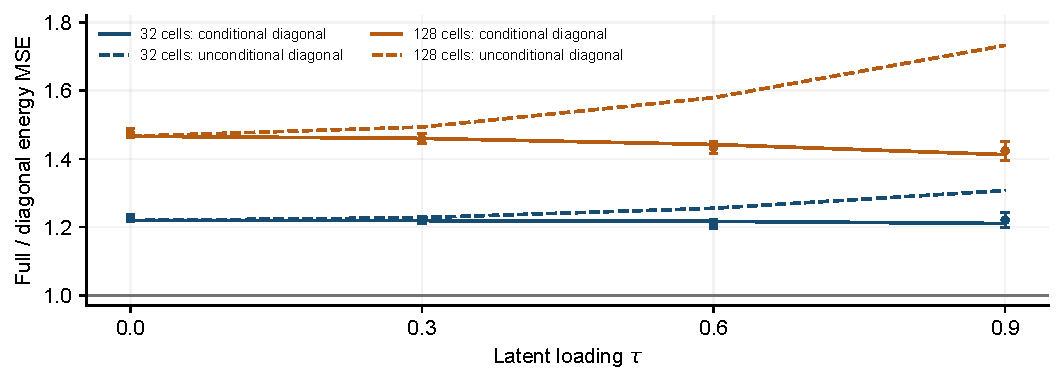
\includegraphics[width=\linewidth]{revision/experiments/latent_correlation_sweep.pdf}
\caption{Common-factor sensitivity at seven bits per source value.
Solid curves retain the full latent mean response in the diagonal comparison;
dashed curves also remove unconditional off-diagonal covariances. Markers
and nominal $95\%$ intervals use independent source vectors.}
\label{fig:latent-sensitivity}
\end{figure}

\subsection{High-contrast diffusion and spatial bit placement}
\label{sec:revision-highcontrast}
We next use $-\nabla\cdot(\alpha\nabla u)=f$ on the same $16^2$ grid,
where $\alpha=0.01$ inside $(x-0.7)^2+(y-0.3)^2\le0.05$ and
$\alpha=1$ elsewhere. Harmonic face conductivities, including the
Dirichlet boundary faces, define the symmetric positive definite operator.
The low-conductivity region is separated from the source hotspot, so the
compression objective accounts for spatial response as well as source scale.
Using the independent hotspot source of Section~\ref{sec:revision-elliptic2d}
and $7$ bits per cell, we retain all
$14$ prescribed codecs and $30\,000$ paired source vectors. At length
$32$, the full-energy rule changes two precision blocks relative to Source
placement: it moves the extra-bit strip from $x\approx0.06,0.12$ toward
the low-conductivity region at $x\approx0.76,0.82$
(Figure~\ref{fig:revision-highcontrast-maps}). This reduces measured RMS by 19.97\%
(paired $95\%$ interval $[19.57,20.37]\%$); at length $128$,
the reduction is 11.25\% ($[10.34,12.17]\%$).
Table~\ref{tab:revision-highcontrast} gives the contiguous results;
both layouts and coincident maps remain in the package. The nominal intervals
contain 13 of $14$ population RMS predictions, with maximum
discrepancy 0.51\%. We also solve $100$ paired sources per codec
by Jacobi-preconditioned conjugate gradients at tolerance $10^{-11}$.
Since $A\succeq0.01A_{\rm Poisson}$, the preceding residual certificate
uses $0.01\lambda_{\min}(A_{\rm Poisson})$; its largest relative bound is
$8.4\times10^{-9}$, while PCG and direct-solve energy values agree within
$4.7\times10^{-11}$ relatively.

\begin{figure}[tb]
\centering
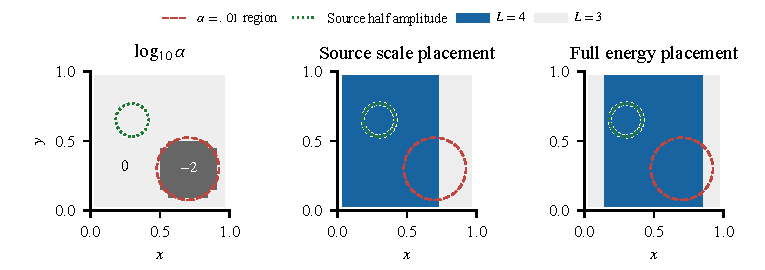
\includegraphics[width=\textwidth]{revision/experiments/highcontrast_precision_maps.pdf}
\caption{The prescribed diffusion coefficient and two length-$32$ contiguous
precision maps. The red disk marks the low-conductivity region; the green
outline is the half-amplitude source contour. Both maps have six blue
$L=4$ blocks and two gray $L=3$ blocks at the same storage cost.}
\label{fig:revision-highcontrast-maps}
\end{figure}

\begin{table}[tb]
\centering
\caption{High-contrast diffusion, $16^2$ sources and exactly $1792$ payload
bits. All entries use contiguous blocks; relative energy RMS is in percent.}
\label{tab:revision-highcontrast}
\begingroup\footnotesize\setlength{\tabcolsep}{5pt}
\begin{tabular}{rlrrr}
\toprule
$|B|$ & Placement & Exact & Ind. & MC $95\%$ interval\\
\midrule
8 & Uniform & 3.213 & 3.159 & [3.202,3.243] \\
32 & Uniform & 4.060 & 3.845 & [4.039,4.103] \\
32 & Source & 3.887 & 3.735 & [3.870,3.925] \\
32 & Energy & 3.114 & 3.005 & [3.099,3.139] \\
128 & Source & 8.948 & 7.993 & [8.817,8.991] \\
128 & Energy & 7.916 & 6.761 & [7.824,7.978] \\
\bottomrule
\end{tabular}\endgroup
\end{table}

\subsection{Calibration from a separate source sample}
\label{sec:revision-calibration}
The preceding high-contrast experiment assumes the source law is known. We
now separate law fitting from codec validation on the same fixed $16^2$
operator. For each $T\in\{32,128,512,2048\}$ and five independently labeled
training samples, we fit $\log b_i=\ell_i+\sigma Z_i$ by coordinate-wise
means and one pooled residual scale. The fitted $(\ell_i,\sigma)$ determine
the source-scale and full-energy bit maps; each map is frozen before a common
30,000-vector validation stream is generated. The uniform map, the oracle
map obtained from the known law, and every learned map are retained; the
validation stream is never used to choose a map.

\begin{table}[tb]
\centering
\caption{Validation RMS and regret for the learned $32$-cell contiguous
maps. Values are medians over five training replicates; regret is relative
to the fixed oracle full-energy map, in percent.}
\label{tab:revision-calibration}
\begin{tabular}{rllrr}
\toprule
$T$ & Source RMS & Energy RMS & Source regret & Energy regret\\
\midrule
32 & 4.498 & 3.100 & 45.07 & 0.00 \\
128 & 3.956 & 3.100 & 27.58 & 0.00 \\
512 & 3.956 & 3.100 & 27.58 & 0.00 \\
2048 & 3.890 & 3.100 & 25.46 & 0.00 \\
\bottomrule
\end{tabular}
\end{table}

The full-moment energy map has median regret 0.00\% at $T=2048$
and 0.00\% at $T=32$; its central 95\% replicate quantile range at $T=32$ is
$[0.00,1.38]\%$. The fitted source scale converges with
$T$ (median log-scale RMSE 0.1714 at $T=32$ versus 0.0222 at
$T=2048$). The median validation error of the train-only full-moment
prediction is -5.43\% at $T=32$ and -1.01\% at $T=2048$.
The fitted energy map recovered the oracle map in 17 of the
20 training fits; the other maps and their validation outcomes are retained.
The validation stream evaluates six unique maps (43 candidate records,
including repeated maps), and all $20$ fits, $40$ learned maps, predictions,
validation energies, and bootstrap intervals are retained. The nominal
intervals contain all six unique-map predictions; repeated candidate rows
are bookkeeping records rather than independent validation tests. The
validation stream is independent of every earlier experiment.

